\chapter{Developer documentation}
\label{ch:impl}

For this project a high level programming language was needed which can support dynamic typing for creating easy statements and storing
lot of different data, the language also has to support runtime interpretation so the user defined statements can be used without
creating a whole new programming language and compiler for it. For these reasons JavaScript with the node.js runtime was chosen. 

\section{Architectural Overview}

The toolkit is heavily depends on the libgit2 \cite{libgit2} library which is a portable, pure C implementation  if the Git core methods,
this library has a version for JavaScript and Node.js which is the nodegit\cite{nodegit}.
The whole toolkit architecture can be represented with the following diagram:

\begin{figure}[H]
	\centering
	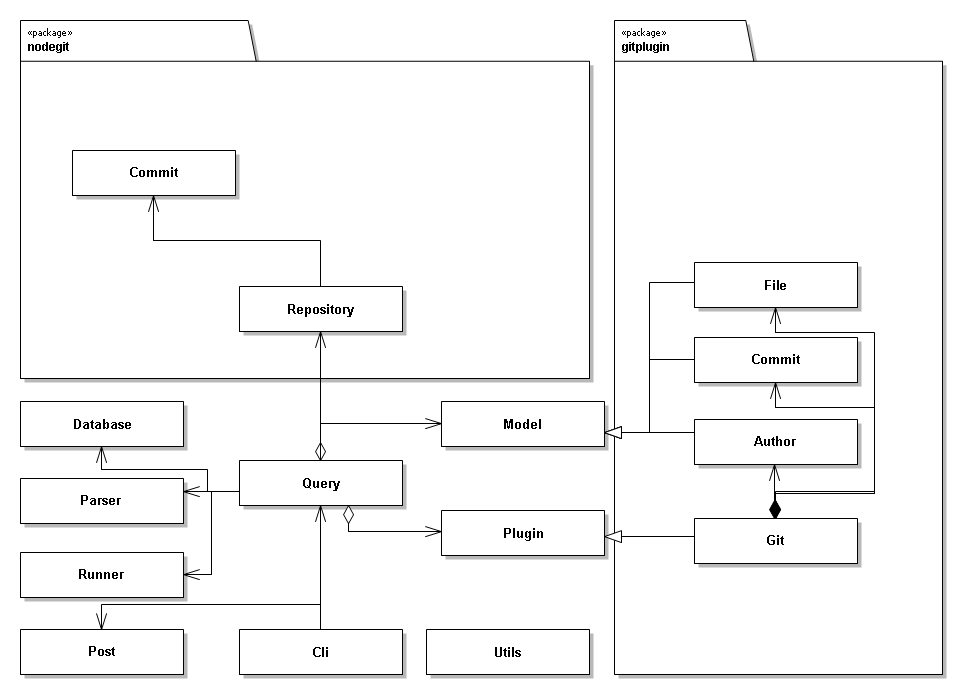
\includegraphics[width=350px]{uml}
	\caption{TODO}
	\label{fig:fig-help}
\end{figure}

The \textit{Query} class is responsible to connect all the modules altogether and also for the IO operations. The query also also
responsible for reading the history from the repository and passing it to the plugins for parsing. The parse data will be stored
in the \textit{Database}. Before the parsing happens the input script also has to be recognized which is done by the \textit{Parse}
module. After both of them is ready the \textit{Runner} module will run the query based on the script and database.

\subsection{Database}

We need to somehow store all the data coming from the parser and plugins. We can assume that the plugins will reduce the size of the
pure data from the repository history. So to provide maximum performance for the query we can use an in-memory database. 
We can also assume that the database will be immutable after the parsing is done. 

The database is collections of hash maps based on the models. The hash map keys are defined by its model \textit{key()} method.
The reason behind this database structure is in the join mechanism in the query. The hash map is implemented with the built in 
\textit{Map}\cite{map} in JavaScript which has access to a given key by a time and space complexity of:

\( O(1) \)

In this way if we connect two models where at least of the models field is a key then we can assume that:\newline
If: N is the count of records by the A model, M  is the count of records by the B model. Then:
	
\(O(N * M) \Leftrightarrow O(N * 1) \Leftrightarrow O(N)\)

\begin{figure}[H]
	\centering
	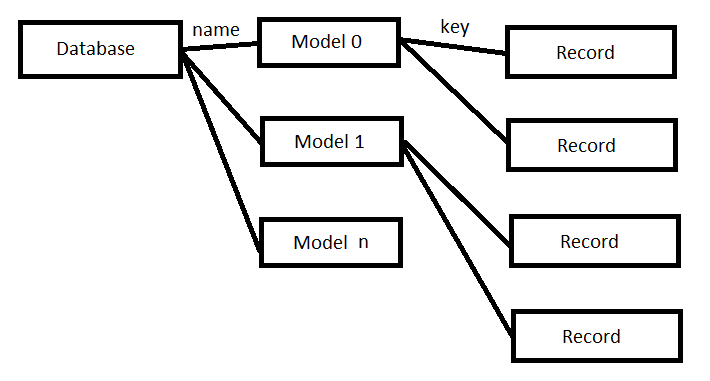
\includegraphics[width=350px]{database}
	\caption{Structure of the database}
	\label{fig:fig-help}
\end{figure}

\subsection{Extensions}

As discussed in the Extending with plugins are the way to add more features to extensions to the toolkit.
Let's look at the included basic \textbf{Git} plugin and its models \textbf{Commit}, \textbf{Author}, \textbf{File}.
This plugin will do the most basic parsing for the histroy which is to extract the commits, the authors, and the files
in the project.

What is needed to make a plugin:
\begin{itemize}
	\item \textit{init()} - The init will be called when repository is opened.
	\item \textit{parse(db, commit)} - This will be called for each commit, the database is expossed as a \textbf{Observer pattern}
	\item \textit{post()} - This will be called when all the commits are parsed
\end{itemize}

The commit in the \textit{parse(db, commit)} is defined in the libgit2 plugin.

The plugin also provided information about itself and what models brings to the database. 
The models will be loaded into database before \textit{init()} is called.

\subsubsection{Functions}

Functions are help for the user to predefined some often used functions for the given plugin.
For example: we may only need a short id for the commit so we can call \textit{short(sha)} inside our query expressions.
Behind the scene this will be injected into the sandbox where the expressions are evaluated.

To define a new functions just pass the function in an array in the \textit{functions()} method.

\subsubsection{Reductors}

Reductors are similar to Functions but its only can be used if a grouping is presented in the query. This will
run for each record in that group. The reductor should be a function and has 2 parameter \textit{reductor(acc, obj)}.
The \textit{acc} will accumulate the result and the object will be the record itself.

To define a new reductor just pass the function in an array in the \textit{reductors()} method.

\subsubsection{Model}

A model is simply defining the structure of data it has two major function \textit{parse(input)}, \textit{parse(key)}. 
This will take the input and transform it that way the database is storing them. 
\textit{name()} will be the name how it can be refereed in the from tag.

Lets look at the Git plugin:

\lstinputlisting[caption={plugins/git.js}]{../plugins/git.js}

\subsection{Parsing and validating scripts}

The one of the most important step is properly read and process the input
from the user script file. Storing this data in the right structure is a key
to speed up the process of the parsing and running the query.

The input script file is a YAML\cite{yaml} which is a human readable data-serialization language. Because the script file structure is declarative
this markup language is ideal. The actual parsing of the YAML file is done by
a third party library from npm which is the yaml\cite{yaml-pck} package.

After parsing the input file into a JavaScript Object the real parsing begin: 

The core tags of script file are the \textit{From}, \textit{Select}, \textit{Where}, all of them is required.

\subsection{From}
The used models should be enumerated here and separated with a \textit{;} character. The parser will create an Object in the \textit{Query} which will map each rename to a model.

 \begin{figure}[H]
 	\centering
 	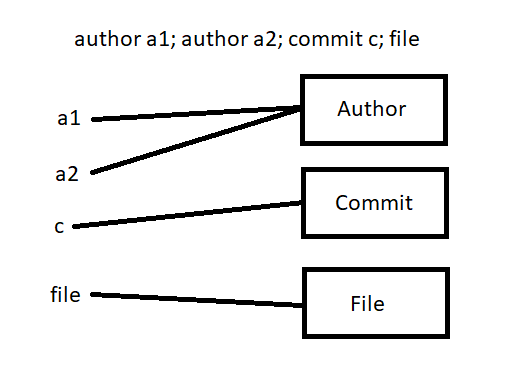
\includegraphics[width=350px]{fromconn}
 	\caption{Structure of the parsed From tag}
 	\label{fig:fig-help}
 \end{figure}

\subsection{Select}
Here the selected \textit{model.field} should be provided with a \textit{;} 
separator character. The \textit{\$} wildcard can be used to select all the
available fields. This can be mixed with a custom transformation of a field.

Here JavaScript statements can be provided which will be evaluated when the
Query runner stops. The statement is transformed by these rules:

\begin{itemize}
	\item If a model with a field is present it will be replaced with a special expression: \textbf{\_\_o['model.field']}
	\item If a plugin provided function is present it will be replaced with: \textbf{\_\_f.function(args)}
	\item If a plugin provided reductor is present it will be replaced with: \textbf{\_\_r.reductor(args)}
\end{itemize}

You can provide multiple field for one selection but you can add without any of it. The header of the selection
will be always the provided statement.

The transformation of the statement is needed because later on when \textit{Runner} start to process the script
it will transform each and every JavaScript statement into a function by:

Creating a lambda expression of the statement: 

 model.field + 2 + fun(4)\newline 
 To:\newline
 (\_\_o, \_\_f) => \{ return \_\_o['model.field'] + 2 + \_\_f.fun(4) \}\newline

This can be cached into the memory so when it has to be evaluated for each record this can speed up the process.

The same principles applies for all the JavaScript statements in the input file, only the \textit{Where} tag makes an exception. 

Note: The JavaScript will be executed in a sandbox mode no node.js module is
available. 

\subsubsection{Where}

In the where tag two parsing is happening: The join and where. Both the where and join are part of the \textit{Runner} workflow. Lets look at this statement, where we are using the the following models: commit c1, commit c2, commit c3

\( c1.sha ==\ '5b2c7'\ \&\&\ c2.sha == c1.sha\ \&\&\ c3.sha == c1.sha\)

Now lets convert this statement into a logic expression where we want to specify the required
data set:

\( \forall{c1}\forall{c2}\forall{c3}(c1.sha ==\ '5b2c7' \wedge c2.sha == c1.sha \wedge c3.sha == c1.sha)\)

Lets simply the expression by:

\( \forall{c1}(c1.sha ==\ '5b2c7') \wedge \forall{c1}\forall{c2}(c2.sha == c1.sha) \wedge \forall{c1}\forall{c3}(c3.sha == c1.sha)\)

Now lets replace the universal quantifier with predicates and we get:

\( P(c1) \wedge G(c1,c2) \wedge H(c1,c3)\)

In this way we can break up the expression into smaller pieces so the parts can be evaluated
without the fully fledged record. This will be important later on...

Before we parse the \textit{Where} flag we are replacing the joins with placeholders.
As discussed in the User Documentation if one of the \textit{model.field} is a key then
we can make faster the \textit{Runner} by using the Maps in the \textit{Database}.

We can assume that all the joins will be done during the run so we can replace these with a
\textbf{true} expression. The join will be stored in a special Object in the Query which will
be used by the \textit{Runner} itself.

\subsection{Parsing Git histroy}

Before talking about how the history is evaluated into a user readable output. Lets take a look
how the history parsing. This part is done by the main \textit{Query} class with the loaded
plugin. First the repository is loaded either by cloning it from Github or by loading a local copy of it. After that if the script file contain the main commit sha then the commit will be the starting point of the algorithm if not them the master commit will provide the starting point.

The history walker algorithm is based on a breadth-first search.

\begin{algorithm}[H]
	\caption{History walker} 
	\label{alg:ibb} 
	\textbf{\underline{function}} load($Plugins$ ,$Repository, commit$)
	\begin{algorithmic}[1] % display line numbers before every n line, here n = 1
		\For{all $plugin$ in $Plugins$}
		\State plugin.setup()
		\EndFor
		\State let Q be a queue
		\State label commit as explored
		\State Q.enqueue(commit)
		\While{( ${\cal Q}$\ is\ not\ empty )}
		\State $c$ := $Q$.dequeue()
		\For{all edges from $v$ to $w$ in $Repository$.parents($v$)}
		\If{$w$ w is not labeled as explored }
		\State label w as explored  
		\State Q.enqueue(w) 
		\For{all $plugin$ in $Plugins$}
		\State plugin.fetch($w$)
		\EndFor 
		\EndIf
		\EndFor
		\EndWhile
		\For{all $plugin$ in $Plugins$}
		\State plugin.post()
		\EndFor
		\end{algorithmic}
\end{algorithm}

After finishing the parsing the Database is locked and can be considered as an immutable object. 

\newpage

\subsection{Running the query}

(2)

\section{Tools}

(1)

\subsection{Gitub}

\subsection{VS Code}

\section{Testing}

(0.5)

\subsection{Unit tests}

(2)

\subsection{Integration tests}

(2)

\chapter{Runtime measurement}
\label{appx:simulation}

(3)